%==========================================
%
% Academic thesis template
%
% Based on KOMA-Script book class.
%
% This template is not officially endorsed 
% by any educational institution.
%
% Ben Swift   22/6/12
% benjamin.j.swift@gmail.com
% http://github.com/benswift/thesis-template
%
% This template is in the public domain
%
% Strongly modified by Veit Heller
%
%==========================================
% preamble
\documentclass[oneside,11pt,xetex]{scrbook}
\KOMAoptions{%
  headings=normal,
  captions=rightbeside,
  bibliography=totoc,
  listof=totoc}

\usepackage{amsmath}
\newcommand{\argmax}[1]{\underset{#1}{\operatorname{argmax}}}
\usepackage{tikz}
\usepackage{pgfplots}

\usepackage{fontspec}
\setmonofont[Scale=MatchLowercase,Mapping=tex-text]{Tahoma}

\usepackage{booktabs}
\usepackage{tabu}
\usepackage{listings}
\usepackage{minted}

\DeclareGraphicsExtensions{.pdf,.png,.jpg}
\graphicspath{{./figures/}}

\usepackage[margin=10pt,labelfont=bf]{caption}
\usepackage[labelformat=simple]{subcaption}
\renewcommand\thesubfigure{(\alph{subfigure})}

\usepackage{metalogo}
\usepackage{hologo}
\usepackage{verbatim}
\usepackage{setspace}
\usepackage{enumitem}

\newlist{transcriptlist}{description}{1}
\setlist[transcriptlist]{font=\sffamily\bfseries,
                              align=left,
                              leftmargin=1.6cm,
                              labelindent=\parindent, 
                              labelwidth=*}

\newenvironment{transcript}%
{\small\begin{transcriptlist}}%
{\end{transcriptlist}}

\newlist{headinglist}{description}{1}
\setlist[headinglist]{font=\sffamily\bfseries, 
                           leftmargin=0cm,
                           style=nextline}

\usepackage[%
backend=biber,
natbib=true,
backref=true,
citecounter=true,
dashed=false,
backrefstyle=three,
citestyle=authoryear-icomp,
firstinits=true,
maxcitenames=2,
maxbibnames=10,
uniquename=mininit,
bibstyle=authoryear,
url=false,
doi=false]{biblatex}

\AtEveryBibitem{\clearfield{month}}
\AtEveryCitekey{\clearfield{month}}

\nocite{*}
\addbibresource[datatype=bibtex]{thesis.bib}

\usepackage[english=british,threshold=15,thresholdtype=words]{csquotes}
\SetCiteCommand{\parencite}

\newenvironment*{smallquote}
  {\quote\small}
  {\endquote}
\SetBlockEnvironment{smallquote}

\usepackage[%
unicode=true,
hyperindex=true,
bookmarks=true,
pdftitle={Beyond .*Script},
pdfauthor={Veit Heller},
colorlinks=false,
pdfborder=0,
allcolors=DarkBlue,
pdfpagelabels,
hyperfootnotes=true]{hyperref}

\usepackage{bookmark}

\usepackage[%
acronym,
nomain,
toc=true]{glossaries}

\usepackage{cleveref}

\newacronym{ast}{AST}{Abstract Syntax Tree}
\newacronym{ajax}{AJAX}{Asynchronous JavaScript and XML}
\newacronym{midi}{MIDI}{Musical Instrument Digital Interface}
\newacronym{html}{HTML}{Hypertext Markup Language}
\newacronym{css}{CSS}{Cascading Stylesheets}
\newacronym{dsl}{DSL}{Domain-Specific Language}
\newacronym{bsd}{BSD}{Berkeley Software Distribution}
\newacronym{zeps}{zeps}{zepto Package System}
\newacronym{zpr}{ZPR}{zepto Package Registry}
\newacronym[plural={Scheme Requests For Implementation (SRFIs)}]{srfi}{SRFI}{Scheme Request For Implementation}
\newacronym{pep}{PEP}{Python Enhancement Proposal}
\newacronym{eep}{EEP}{Erlang Enhancement Proposal}
\newacronym{r5rs}{R5RS}{Revised\textsuperscript{5} Report on the Algorithmic Language Scheme}
\newacronym{jit}{JIT}{Just In Time Compiler}
\newacronym{llvm}{LLVM}{Low Level Virtual Machine}
\newacronym{frp}{FRP}{Functional Reactive Programming}
\newacronym{gui}{GUI}{Graphical User Interface}
\newacronym{ir}{IR}{Intermediate Representation}
\newacronym{ghc}{GHC}{Glasgow Haskell Compiler}
\newacronym{repl}{REPL}{Read-Eval-Print Loop}
\newacronym{ffi}{FFI}{Foreign Function Interface}
\newacronym{api}{API}{Application Programming Interface}
\newacronym{dom}{DOM}{Document Object Model}
\newacronym{w3c}{W3C}{World Wide Web Consortium}
\newacronym{yui}{YUI}{Yahoo User Interface Library}

\renewcommand{\thepage}{\roman{page}}

\makeindex
\makeglossaries

\linespread{1.3}

\begin{document}

\begin{titlepage}
	\centering
	{\scshape\LARGE Beyond .*Script \par}
	\vspace{1cm}
	{\scshape\Large Implementing A Language For The Web\par}
	\vspace{2cm}
	{\Large\itshape Veit Heller\par}
	\vfill
  A thesis submitted for the degree of \\
  B.Sc. of Applied Computer Science (Fachbereich II) \\
  of the University of Applied Sciences (HTW) Berlin
	\vfill

  \textbf{Supervisory Panel}\\

  Prof. Dr.-Ing. Hendrik \textsc{Gärtner}\\

  Prof. Dr.-Ing. Henrik \textsc{Lochmann}\\
	\vfill

\end{titlepage}

\dedication{\small{\emph{For Meredith, Tobias and all the people who cope with me. Your undying support will not be forgotten.}}}

\pdfbookmark{Title Page}{Title Page}

\frontmatter

\addchap{Abstract}

This thesis presents and evaluates a port of the zepto programming language to the web. It aims to
work as seamlessly with existing technologies as possible and is largely influenced by \gls{r5rs},
a standard of the Lisp derivative Scheme.\footnote{A deeper introduction into \gls{r5rs} can be found
in Section \ref{sec:ExistingStandards}.}

It is the result of over a year of independent research on zepto, a new programming language
targetting various environments. The prototype described here and implemented for this
thesis runs on JavaScript, a language found natively in many web browsers.

The central problem addressed by this thesis is the incoporation of a language runtime
into the web ecosystem. This is achieved without the need for extensive code rewrites
while supporting most features of the reference implementation of zepto, including large
parts of the standard library. This also includes interoperability between the two languages.

It is also discussed in which ways tooling for both JavaScript and zepto, most specifically
their respective package managers, interoperate to build larger scale web applications.

\pdfbookmark{Contents}{Contents}
\tableofcontents

\printglossary[type=\acronymtype,title=Abbreviations]

\mainmatter

\pagestyle{headings}

\setchapterpreamble[u]{%
  \dictum[\emph{B. Kernighan}]{Controlling complexity is the essence of computer programming.}
  \bigskip}
\chapter{Introduction}
\label{chap:intro}

\section{Motivation}
\label{sec:Motivation}

JavaScript has, since its inception, attracted a lot of controversy. This is rooted
in various aspects of its design, from prototypal inheritance and the \gls{dom} to
its operator precedence. Especially prototypal inheritance  has been the cause
of a lot of discussion in the Computer Science community. It has the reputation of
being counter-intuitive, though it is older than JavaScript, the first commonly known
programming language that implemented prototypal objects being Self.

This and a few other design choices have prompted many programmers to develop
wrapper libraries around almost anything that constitutes the language. The most widely-used
example of this is arguably jQuery, a library that abstracts over the \gls{dom}.
But more arcane topics have been covered as well: there is, for example, the \gls{yui}, a now-abandoned
project of Yahoo that aimed to abstract over web \glspl{api} but also came with
its own inheritance model. This model likened JavaScript prototypes to classical classes by
introducing special functions and properties to the objects such as \texttt{extend}
and \texttt{superclass}.

These and other libraries have shaped the way JavaScript has developed. In the
upcoming revisions of ECMAScript\footnote{ECMAscript is the officially trademarked
name for the application developers and browser vendors most commonly refer to as
JavaScript.}, ECMAScript 6\footnote{ECMAScript 6 was renamed ECMAScript 2015
during the standardization process, but this thesis uses the more commonly known name
of the revision for the sake of clarity. For an up-to-date version of this revision
please refer to \parencite{ECMA6}.} and ECMAScript 7\footnote{Now ECMAScript 2017. For
an up-to-date version of the current draft please refer to \parencite{ECMA7}.}, a
lot of conveniences from third-party libraries have been adopted by the
``vanilla''\footnote{A common name for JavaScript that refrains from leveraging
paradigm-altering libraries.} JavaScript canon.
Among these features is the widely controversial introduction of a \texttt{class}
notation for JavaScript that makes prototypes feel more like classes without
breaking from existing semantics.

\subsection{Preprocessors \& Transpilers}
\label{pretrans}

Classes and other features have been available to JavaScript developers for much
longer than the latest iterations of the JavaScript language without them needing
to rely on a possibly massive library - provided they use a preprocessor.
One of the earliest exemplars of preprocessing for JavaScript, CoffeeScript, included
\texttt{lambdas}, a shorthand for anonymous functions; and \texttt{pattern matching},
a technique for destructuring data; and \texttt{classes}, all of which found
their way into the latest ECMAScript revisions.

Preprocessing can serve a lot of different purposes apart from providing
syntactic commodities to the programmer. Babel, for instance, is a relatively
novel library for transpiling JavaScript that adheres to the new standards
of ECMAScript back to older revisions, for the sake of backwards-compatibility.
It also aims to provide small optimizations before the code reaches the compiler,
such as constant hoisting.\footnote{Constant hoisting is a compiler optimization
technique that eliminates pure functions that always produce the same result in favour
of global constants to reduce the overhead of function calls.}

Transpilation from a different language is another increasingly popular
way to use JavaScript as a platform. One could argue that CoffeScript
is nothing short of a transpiler; but one could also argue against this idea,
considering its only purpose is to compile to JavaScript. Other general-purpose
languages such as Clojure and C++, originally developed to run on other platforms,
have the option to compile to JavaScript through ClojureScript \parencite{CLJS} and
Emscripten \parencite{ZAKA}, respectively.

\subsubsection{Caveats}

This thesis was inspired by the work done in the field of transpilation to
JavaScript. Its goal is not to present yet another attempt at transpilation,
but rather to rethink the way languages are incorporated into the web of today.

At their heart, all of the preprocessors and transpilers that target JavaScript
are JavaScript, even if the syntax and semantics differ radically. There needs
to be a clean mapping of the source language to JavaScript. Because of its flexibility,
this is often a doable task, albeit not always desirable.

The value of having the same level of abstraction present at runtime as at compile-time
is obvious if the language that is considered places strong emphasis on code
mutability, such as in Lisp or Elixir\footnote{As exemplified by Chris McCord in
\parencite{ELIX}.}. This thesis aims to equip the programmer with these abstractions
by presenting a language that is not a preprocessor, but a genuine runtime system
for the frontend.

\section{Goals of this Thesis}

The primary goal of this thesis is to present a novel approach at implementing languages
for the Web. This is exemplified by a sample implementation of a non-trivial, pure, and
largely feature-complete functional programming language that has been tested
in production systems.

There are many reasons to use a procedural or objective-oriented language as
a prototype. On one hand, the language itself could be more easily implemented in
JavaScript if it is reasonably close to it. Another point that speaks
against using a functional --- and especially pure --- programming language is the
possibility of making interoperability harder because JavaScript is intrinsically
impure and stateful.

But all of those reasons could also be read as argument \textit{for} the implementation
of a functional language. The difference showcases JavaScript's ability
to express concepts that are foreign to it. It also serves as a better
test bench for more advanced implementation patterns.

This is especially true for those features of the base language that are not
present in JavaScript and non-trivial to add to it from a user perspective.
The features present in the target language implemented in this thesis but not
present in JavaScript most notably include Macros\footnote{The ability to rewrite
code at parse or compile time, see Section \ref{macro}.} and Continuations\footnote{The
control state of a program represented as a data structure within the code, see
Section \ref{continuation}.}. These features were chosen especially because they are
extremely foreign to JavaScript programming.

\section{Structure of this Thesis}

Chapter 2 examines related work in the field of cross-compilation into JavaScript and implementation
of interpreters that are directly embeddable into larger systems.

Chapter 3 gives an overview of the concept design and how the features are laid out to match the needs
of both the goals of this thesis and the prototype itself.

Chapter 4 presents the system design and how the prototype integrates into existing web components.

Chapter 5 discusses the implementation by picking out different fundamental parts of the system and
presenting how they work.

Chapter 6 evaluates the prototype. This includes problems such as how well the integration of the
system worked and how it compares to the reference implementation of zepto.

Chapter 7 gives a brief summary of what was done and an outlook as to what might happen with
both the desktop and the JavaScript versions of zepto in the future.

\chapter{Related Work}
\label{chap:RelatedWork}

This chapter aims to give a quick overview of work that has already been done in the
field of transpilation to and language implementations on top of JavaScript. A few
of the most important specimens have already been mentioned briefly in Section \ref{pretrans}.

\section{Existing Projects}

In this section a brief overview of a short, but not necessarily exhaustive list of
transpilers to JavaScript shall be presented. The source languages include
existing programming languages as well as languages explicitly acting as
a layer of abstraction over JavaScript.

The aim of this section is not to present the reader with the syntax and semantics
of every single language that is discussed. Rather, the idea is to equip them with a
general overview of the ecosystem at the time of writing and how it correlates to
the work presented in this thesis.\footnote{The programming language that is described
in this thesis will be henceforth referenced to as zepto-js.}

\subsection{Transpilers}
\label{trans}

Transpilers are normally defined as being compilers that translate one high level language
into another. They are often referred to as cross-compilers; however, this term is imperfect,
as it also refers to compilation from one hardware platform or operating system to
another.

Due to this ambiguity, the name \textit{transpiler} was chosen to refer to these
kinds of systems in the context of this thesis.

\subsubsection{GHCJS}
\label{sec:GHCJS}

GHCJS --- often hyphenated as GHC-JS --- is a transpiler from the Haskell language
to JavaScript. It is currently maintained by Luite Stegeman. It aims to ``solve
the JavaScript problem''\footnote{A talk given by Stegeman bore this title, see
\parencite{STEG}.}, in that it enables the user to compile any Haskell program to JavaScript.
GHCJS does so by insterting a custom compiler backend into the \gls{ghc} toolchain
that emits JavaScript instead of machine code.

GHCJS is the compiler used in this thesis to transpile the existing zepto codebase
to JavaScript. Its plug-and-play design, near-complete implementation of the
Haskell programming language, and relative maturity all contributed to the decision
to use it as a development platform.\footnote{Further discussion of the design
and decision process can be found in Chapters \ref{chap:ConceptDesign} and
\ref{chap:SystemDesign}.}

\subsubsection{Emscripten}

Emscripten as discussed in \parencite{ZAKA} aims to be a transpiler from \gls{llvm} to
JavaScript. Its primary focus is the translation of C and C++ source code
to JavaScript.

Emscripten's use case is similar to that of GHC-JS, enabling the user to both \blockquote{(1)
Compile code directly into LLVM assembly, and then compile that into JavaScript
using Emscripten, or (2) Compile a language’s entire runtime into LLVM and then
JavaScript, as in the previous approach, and then use the compiled runtime to
run code written in that language (\cite{ZAKA})}. Translating a runtime into
JavaScript for executing foreign code from within JavaScript sounds
suspiciously like what zepto-js is trying to achieve.

In fact, there have been efforts to leverage this potential of \gls{llvm} in
the past. For example, Ryan F. Kelly is trying to make the PyPy \gls{jit}\footnote{A \gls{jit}
designed to speed up Python programs by analyzing and compiling them, described
in \parencite{PYPY}.} work in the browser.\footnote{While this project offers
a live demonstration which can be found on its \href{https://pypyjs.org}{website, accessible
under https://pypyjs.org}, further documentation on it is sparse and there is seemingly
no academically viable source detailing its development and architecture.}

As zepto is written in Haskell, though, \gls{llvm} was not a viable development
platform. If it had been chosen, the goal of reusing the code of the reference
implementation would not have been met.

\subsubsection{ClojureScript}
\label{sec:ClojureScript}

ClojureScript is a backend for the Clojure programming language that targets
JavaScript. Initially developed by Rich Hickey, the author of Clojure, it is
now maintained under David Nolen's lead \parencite{CLJS}.

Being a Lisp, it has obvious syntactic similarites to zepto. Yet, as it is
transpiled rather than interpreted directly in the browser, programming against
it is quite difficult. Specifically, the way the \gls{ffi}\footnote{A \gls{ffi}
is a facility that provides an interface for calling function defined in another
language, often the target or host language of the implementation.} works is quite
different from zepto-js, as ClojureScript has a lot of syntactic integrations
that help embed JavaScript within it. All functions prefixed with a period are
assumed to be JavaScript functions on the prototype of the object provided as
first argument. JavaScript values can be directly accessed through the \texttt{js}
namespace. zepto's design is discussed in Section \ref{sec:ffi}.

\begin{listing}[H]
\caption{A comparison of the \gls{ffi} of JavaScript in zepto and ClojureScript.}
\begin{minted}[linenos]{racket}
; ClojureScript provides syntactic abstractions over
; the embedding of foreign code.
(.getElementById js/document "body")

; An equivalent zepto call, with strings
(js "document.getElementById(\"body\")")
; OR, if a variable is accessed
(js (++ "document.getElementById(\"" body "\")"))
\end{minted}
\end{listing}

\subsection{Abstraction Languages}

The languages mentioned here are languages that abstract purely over JavaScript,
choosing it as their primary backend. This differs from the languages discussed
in Section \ref{trans}, which are general purpose languages with the option to compile
to JavaScript if desired by the developer.

\subsubsection{CoffeeScript}

As mentioned in Section \ref{pretrans}, when it first appeared, CoffeeScript was one of the first transpilers that targeted JavaScript.\footnote{The first git commit
dates back to
\href{https://github.com/jashkenas/coffeescript/commit/8e9d637985d2dc9b44922076ad54ffef7fa8e9c2}{December 13th, 2009} as seen in the
commit history of \texttt{https://github.com/jashkenas/coffeescript}.
The first public release took place shortly after that.} Many of the constructs,
relating both to syntax and semantics, have been adopted by JavaScript.
CoffeeScript is similar to JavaScript in that it is a procedural, prototypal
language. No semantic features have been added or removed from JavaScript\footnote{Although
the syntactic abstractions often make it seem as if CoffeeScript offers
constructs that are missing from JavaScript.}, making it relatively
dissimilar to the programming system presented in this thesis.

The biggest deviations from JavaScript can be found in the syntax.
The syntax of CoffeeScript is influenced by both Python and Ruby \parencite{COFF}.
For instance, contrary to JavaScript, indentation is significant, and
comments start with a pound symbol. These changes are supposed to simplify
the development process.

\subsubsection{Elm}

Elm as it is presented in ``Elm: Concurrent FRP for Functional GUIs''
is a language centered around \gls{frp}\footnote{An in-depth
explanation of \gls{frp} is outside of the scope of this thesis.
\gls{frp} is a programming style for user-centric programs first described
in Paul Hudak's and Conald Elliott's 1997 paper ``Functional Reactive
Programming'' \parencite{FRP}.} with a special regard to browser-based
\glspl{gui} \parencite{CPL}. It borrows its syntax largely from Haskell
and is a pure, functional programming language. Notable features include
\gls{gui}-centric tooling, such as a ``time-traveling'' debugger that caches
the state of a program at any given time, allowing for rewinding, forwarding,
and jumping.

Elm's sole similarity to zepto-js is that it is a functional language for the Web.
However, unlike zepto-js, it compiles to JavaScript, \gls{html} and \gls{css}, and
once again falls short of actually getting the code to the browser. It is also very
centered around \gls{frp}, whereas zepto-js aims to be a general-purpose programming
environment. Therefore, Elm's relation to this thesis is merely tangential, but the
advances made by it are important for the context in which zepto-js is placed.

\subsubsection{PureScript}

PureScript is, much like Elm, a functional, pure programming language
that borrows a lot of its syntax from Haskell. It aims to compile into
human-readable JavaScript and make possible general purpose programming
for the web in a strongly typed, functional style.

It is different from GHCJS in that it does not provide compatibility
with Haskell code, although many libraries and functions are relatively
similar.\footnote{See Listing \ref{fig:ps} for an example.}

As it shares a lot of features with Elm, it also largely shares its
differences to zepto-js.

\begin{listing}[H]
\caption{A juxtaposition of a simple function in Haskell and PureScript.}
\begin{minted}[linenos]{haskell}
-- | Extract the first element of a list (as implemented in the language standard library).
-- | The Haskell version is unsafe and will throw an error
-- | if it encounters an empty list.
head :: [a] -> a
head (x:_) =  x
head [] =  badHead -- an exception function

-- | the list data type in PureScript is safe by design and
-- | the function returns a Maybe monad.
head :: forall a. List a -> Maybe a
head Nil = Nothing
head (Cons x _) = Just x
\end{minted}
\label{fig:ps}
\end{listing}

\section{Existing Standards}
\label{sec:ExistingStandards}

When developing a programming language derived from the Lisp family, one builds on
top of almost seventy years of development, formalization, and research. Of course
many of the standards formed during this time are now obsolete.
Nonetheless, the effort of standardizing the many languages and implementations
is still thriving.

Over the years, two main categories of languages have developed: Common Lisp
and Scheme. While the syntactic proximity remains, the categories differ
widely conceptually. Figure \ref{fig:lispcomp} shows the differences between
those language families.

zepto is a Scheme derivative loosely based on \gls{r5rs} \parencite{R5RS}, the most
widely implemented standard of Scheme. It draws from a lot of standard library
functions, syntax definitions, and continuations, but aims to introduce custom namespaces
to provide a cleaner, more modular way of defining software libraries.\footnote{This module
system will be explained in Chapter \ref{chap:ConceptDesign} in depth.}

The reason for which a Scheme derivative was chosen over an implementation of Common Lisp
can be found in the feature set (see Figure \ref{fig:lispcomp}); hygienic macros and
continuations are valuable abstractions that guarantee that components work
together.\footnote{An example of code that works as expected in Scheme but not in
Common Lisp is presented in Listing \ref{fig:schemevscomlisp}.} It
implements a simple – if a bit contrived – version of binary \texttt{or} in Common Lisp and
in Scheme. In Common Lisp, the variables defined in regular code will potentially be
shadowed by the ones generated during macro expansion, whereas in Scheme they reside in
different contexts and are thus hygienic. This renders the system more intuitive and eliminates
a class of potential bugs, making it more desirable.

While \gls{r5rs} is certainly a valuable standard and provided a lot of very useful information
for the development for zepto, the language is not as closely tied to the standard as most other
implementations. This allowed for the development of zepto-js to progress mostly unencumbered by
incompatibilities, although one goal of the development effort was not to break any existing
syntactic or semantic ties with \gls{r5rs}. Disrupting these links could potentially have broken
a big part of the standard library, with the library being one of the major arguments for zepto's
existence as a language.

\begin{center}
\begin{figure}
  \begin{tabu}{| l | l | l | l | l | l |}
  \hline
  \rowfont{\footnotesize}
              & Macro Keyword & Macro Dispatch   & Hygienic Macros & Continuations & Standard\\ \hline
  \rowfont{\footnotesize}
  Scheme      & define-syntax & pattern matching & present         & present       & ANSI Common Lisp\\ \hline
  \rowfont{\footnotesize}
  Common Lisp & defmacro      & argument passing & not present     & not present   & RNRS\\ \hline
  \end{tabu}
  \caption{A comparison between Common Lisp and Scheme}
\label{fig:lispcomp}
\end{figure}
\end{center}

\subsection{\glspl{srfi}}

\glspl{srfi} comprise an important argument for adhering to the \gls{r5rs} standard. They are
standard library enhancement proposals from the Scheme programmer community that suggest
enahcements through the addition of features, much like \glspl{pep} for the Python
programming language and \glspl{eep} for Erlang. However, the difference that sets SRFIs
apart from the latter two is the inclusion of a reference implementation.\footnote{This
is not required, but part of the ``good tone'' of the community, and \gls{srfi}s lacking them
are relatively rare.} zepto currently supports five of these requests by default,
one of which implements a core feature of the language: descriptive custom data types, better
known as smart structs.

In the past, the relative ease of porting the implementation of these requests was a major
convenience. By moving even uurther away from the Scheme standards, this process would
undoubtedly be affected in a negative manner. Even mere renaming incurs the cost of finding
and replacing all occurrences of the affected name, which leads to a new class of potential
bugs. Thus, for both the reference implementation and its
JavaScript equivalent, a core set of primitives must be available under all circumstances
to allow for the cross-fertilization of Scheme and zepto.

\begin{listing}[H]
\caption{Common Lisp Macros vs. Scheme Macros}
\begin{minted}[linenos]{scheme}
; the Common Lisp version
(defmacro my-or (x y)
  `(let ((tmp x))
    (if tmp
      x
      y)))

(my-or #f #t)
; works (yields true), expands to:
(let ((tmp #f)) (if #f #f #t))

(let ((tmp #t))
  (my-or #f #t))
; does not work (yields false), expands to:
(let ((tmp #t)) ((tmp #f)) (if #f #f tmp))

; the Scheme version
; it will work as expected in both examples
(define-syntax
  (syntax-rules
    ((my-or x y)
      (let ((tmp x))
        (if tmp
          x
          y)))))
\end{minted}
\label{fig:schemevscomlisp}
\end{listing}

\subsection{Unix}

While not necessarily a standard, Unix and its guidelines do indirectly affect zepto. Much of zepto's
tooling, such as the \gls{zeps} use Unix utilities and system calls internally. This is expected to change
in the future, but so far all of the developers who have worked on or with zepto\footnote{To the
best of the author's knowledge.} have used Unix or Unix-like systems such as MacOS X or \gls{bsd}.
This is less of a problem in the browser context because many of the packaging and versioning
tools are run from the command line before the application is distributed. It is important to
keep in mind, though, that some of the tools rely on a specific Operating System when
developing zepto programs.

\setchapterpreamble[u]{%
  \dictum[\emph{Larry Wall}]{Take Lisp, you know it's the most beautiful language in the world -- at least up until Haskell came along.}
  \bigskip}
\chapter{Concept Design}
\label{chap:ConceptDesign}

The concept of a version of zepto that would run on JavaScript arose rather
naturally from the work done on zepto as a backend-agnostic, run-everywhere
concept language. Concurrently to the work on a nanopass compiler that
targets \gls{llvm} and Erlang but supports pluggable backends by design, efforts
have been made to bring the language into the browser setting. After preliminary
work on a compiler backend that emits JavaScript was discarded in the
early stages of its development for the reasons stated in Section \ref{sec:Motivation},
the idea presented in this thesis emerged.

In the following, a brief overview of the design of the concepts used
in the port and how they impacted the construction of the system will be
discussed. A system-based design overview is presented in Chapter \ref{chap:SystemDesign}.

\section{Construction Design}
\label{sec:ConstructionDesign}

The value of integrating zepto into existing web infrastructure lies in
the addition of a host of new features that are not present natively in
JavaScript and hard to implement in a stable manner.\footnote{While stability
is not guaranteed by the current version of zepto, it is tested and deployed
in production systems and seems to function rather reliably.}  The goal of
the prototype was thus to expose all of the features that define zepto in
the JavaScript implementation as well.

An explanation as to why a Lisp was chosen for this thesis --- and specifically
zepto --- shall be given in the following.

\subsection{Lisp}

A common saying among programming language designers is that every programmer has written
their own implementation of Lisp.\footnote{The README of the femtolisp project even goes so
far as to claim ``Some programmers' dogs and cats probably have their own lisp implementations
as well.'' \parencite{BEZL}.} There are a lot of different implementations of Lisp
in the wild, even ones that compile to JavaScript, such as ClojureScript, the
backend for Clojure referenced in Section \ref{sec:ClojureScript}.

The language's simplicity on a parsing level contributes to its popularity as
a language to implement.
A simple Lisp can be implemented in fewer than one hundred lines of code if no
intermediate representation is generated. This is made possible by Lisp's unique property
of enclosing every statement in parentheses, in which the first element within
those parentheses is the statement name and the other elements are the arguments.
Each of these units is called an S-Expression --- a shorthand for ``symbolic expression'' ---
and they are often represented as nested lists, although this is an implementation detail.
It can be evaluated straight from a textual level, because problems such as operator precedence
and statement ambiguity do not exist. In regular Lisp, as specified in the initial paper by
John McCarthy, only a of handful special forms are required for Turing-completeness, as well
as expressiveness and elegance \parencite{JCM}.

\subsection{zepto}
\label{ququ}

As explained in Section \ref{sec:ExistingStandards}, zepto is a new Scheme implementation. It seeks
to be as small as possible, to be able to target a lot of different backends and simplify the
process of writing new backend code. Currently, \gls{llvm} and Erlang Core\footnote{Erlang Core 
is the \gls{ir} of Erlang code before it is complied. Resources and documentation
about it are sparse; it mostly seems to exist inside the BEAM's implementation. A small
paper \parencite{ERL} that describes its basics was used to implement the compiler from
zepto.} bindings are under development. zepto's reference implementation is a simple interpreter
that evaluates code directly from the \gls{ast}. This is slow but ensures a small
interpreter size.\footnote{The entire codebase is only about 4000 lines of Haskell code.}
The compilers are written directly in zepto itself.

The small code base makes zepto a good target for porting it to the web. Furthermore, because
it is written in Haskell the code base was expected to be almost entirely compilable
to JavaScript using GHCJS\footnote{GHCJS is the transpiler mentioned in Section \ref{sec:GHCJS},
a backend for the \gls{ghc} targetting JavaScript instead of native code.}. It offers many
advanced compilation features such as inlining of JavaScript into the Haskell code
base using a technique called quasi-quoting, wherein a special character sequence delimits the
inlined code, much like regular quotes. This tool set was expected to simplify the work of
porting an existing language to the web.

Of course there are other reasons to use a functional language to demonstrate how to
bring a language into the browser. With both syntax
and semantics differing greatly from JavaScript, this example enables languages more
closely related to JavaScript to eventually make their way into the browser.

\subsection{Macros}
\label{macro}

Macros are a mechanism for rewriting code at compile time. As discussed in
Section \ref{sec:ExistingStandards}, zepto's macros are hygienic, which prevents name collisions
with code at runtime and eliminates a class of particularly nasty bugs. Macros are
evaluated in a step between the parser and the actual compilation of code
called macro expansion, in which the compiler rewrites parts of the source code that reference
it according to its specifications.

Because Scheme macros leverage pattern matching and argument overloading by default,
they allow for syntactic extensions of the language. An example for a simple yet
interesting case is made in Listing \ref{fig:listcomp}, where a simple syntactic rule set
for list comprehensions is defined, not unlike a \gls{dsl}, albeit a very small one.
This particular list comprehension is syntactically close to the same construct in
Haskell, although the semantics should be relatively clear at a close inspection and
are, for the sake of example, a bit simpler than in the language by which it is inspired.

\begin{listing}[H]
\caption{Defining \& using a macro in zepto}
\begin{minted}[linenos]{scheme}
; this defines a macro of the name listcomp
(define-syntax listcomp ; the name
  (syntax-rules (<- |) ; the set of rules and special tokens to respect
    ((_ expr | elem <- elems) ; the pattern to match where
                                   ; the underscore character is a wildcard
      (map (lambda (elem) expr) elems)))) ; the pattern is simply rewritten to a call to the map function

; add1 to every x in the list
(listcomp (add1 x) | x <- [1 2 3 4]) ; rewritten to: (map (lambda (x) (add1 x)) [1 2 3 4])
(listcomp (add1 x) | x <- (range 4)) ; rewritten to: (map (lambda (x) (add1 x)) (range 4))
\end{minted}
\label{fig:listcomp}
\end{listing}

It should be noted that zepto supports list comprehensions by default and they are
both a bit more concise and more powerful --- as they allow for the filtering of
elements from the source list --- than the version defined here.

\subsection{Continuations}
\label{continuation}

Continuations are a datatype representing the state of a program at the time of
request, including environments, definitions, and execution path. By manipulating
it and injecting it into different contexts, it becomes a powerful tool to switch
back and forth between multiple threads of execution, without actually creating
or managing threads. A practical application of coroutines was for instance
presented in ``Continuations and Coroutines'', where it was used to implement a fully formed
coroutine system that was capable of starting, stopping, and pausing execution
of multiple coroutines at once without the need for actual threading \parencite{COR}.

An exhaustive explanation of continuations cannot possibly be given in the scope
of this thesis, for further information about this concept refer to ``The discoveries
of continuations'' \parencite{CONT}.

\subsection{The numerical tower}
\label{numbers}

Scheme --- and, for that matter, zepto --- is also known for providing a ``numerical
tower'' to the programmer. It represents a stack of numerical types, each building
on top of the other. Scheme provides infinte precision integers, which means that
these numbers will never overflow; rationals, which are fractions represented by
two integers --- a numerator and a denominator; floating point numbers, which normally
wrap the biggest floating point number type representable by the hardware; and, finally,
complex numbers, which are represented by two floating point numbers, one representing
the real part and the other the imaginary part. zepto includes an additional numerical
type called \texttt{small}, which wraps the biggest hardware type for integer numbers,
for reasons of performance. It is advised to use them only in performance-critical
applications. The numerical tower is presented graphically in Figure \ref{fig:numtower}.

\begin{figure}[H]
\centering
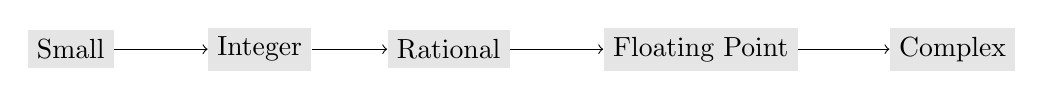
\begin{tikzpicture}
[->,scale=.8,auto=left,every node/.style={rectangle,fill=gray!20}]
  \node (n4) at (14,0)   {Complex};
  \node (n3) at (10,0)   {Floating Point};
  \node (n2) at (6,0)    {Rational};
  \node (n1) at (3,0)    {Integer};
  \node (n0) at (0,0)    {Small};

  \foreach \from/\to in {n0/n1,n1/n2,n2/n3,n3/n4}
    \draw (\from) -> (\to);

\end{tikzpicture}
\caption{zepto's numerical tower}
\label{fig:numtower}
\end{figure}

COercing between these types is always safe when done in the direction denoted
by the arrows in Figure \ref{fig:numtower}. When coercing in the other direction, information
is lost, or, in the case of coercion from floating point numbers to rationals, the meaning
of the statement is ambiguous\footnote{This is due to any finite floating point number
having an infinite number of representations as fractional values.}.

\section{Additional Features}

There are features in zepto that are not present in Scheme as specified by \gls{r5rs}, such
as the module system and the extensive standard library. In this section, a brief list of
the features and libraries that discriminate zepto from ``regular'' Scheme shall be examined.

\subsection{The module system}

zepto implements a custom module system that is completely defined in terms of the language
itself. A small code example of different actions in zepto's module space is presented in
Listing \ref{fig:zepmod}.
This allows for namespaced, conditional, and renaming imports, a feature missing from standard
Scheme.\footnote{Although the latest Scheme standard R7RS included such a mechanism \parencite{R7RS},
it is not widely implemented.}
This approach has a few upsides that all boil down to the module system being available in the
user namespace; monkey-patching and mocking objects is possible, simplifying for instance
testing and fixing flaws in the program at runtime. The module system is also relatively small
and simple, at about 130 lines of macro-backed code, which makes it fairly maintainable.

However, this approach comes not without its drawbacks. Most notably, relying on a module
system that works at runtime requires more complex compilation and a dispatch system to
be present while the program is running. It also requires global data in the form of a
special variable --- named \texttt{*modules*} --- holding the mapping of names to values,
a concept that is unusual for a functional programming language and might hinder the
compilation into other representations. Global data is also normally either not thread-safe
or relatively slow to use if it requires some sort of synchronization mechanism --- which is
not currently a feature that zepto implements.

This is an acceptable tradeoff for the current version of zepto, as all of the
target languages of zepto's compiler support modules. They therefore provide a
suitable representation for the semantics of zepto's system.

In the case of JavaScript, this part of zepto's implementation proved not
to be a problem and worked without further tweaking.

\begin{listing}[H]
\caption{Defining \& using a zepto module}
\begin{minted}[linenos]{scheme}
; this defines a module of the name "mathematics"
(module "mathematics"
  (export
    `("add" ,add)
    `("substract" ,substract)
    `("multiply" ,multiply))

  ; the actual worker function (not exposed)
  ; applies a function to a list of arguments
  (doop (op args)
    (apply op args))

  ; the exported functions; essentially just wrappers
  ; around doop
  (add (lambda arguments (doop + arguments)))
  (substract (lambda arguments (doop - arguments)))
  (multiply (lambda arguments (doop * arguments))))

; will return a reference to the function
(import "mathematics:add")
; so that it can be bound to a name
(define add (import "mathematics:add"))
; or called directly
((import "mathematics:add") 1 2)

; import all under the namespace "mathematics"
(import-all "mathematics")
; import all under the namespace "mt"
(import-all "mathematics" "mt")
\end{minted}
\label{fig:zepmod}
\end{listing}

\subsection{The standard library}

zepto comes with a fairly extensive standard library. It includes a wide
variety of utilities spanning such diverse topics as cryptography\footnote{As found
in the \texttt{rsa} module, which implements RSA key generation, signing,
validating, and en- and decryption.}, testing, monads, parsing command line
arguments, and a parser combinator.\footnote{An exhaustive list of the modules
found in the zepto standard library at the time of writing can be found in appendix
\ref{app:stdlib}.}

This is reasonably unusual for Scheme implementations in that many of them
come with a fairly minimalistic set of libraries that are often based almost
exclusively on SRFIs. Two notable exceptions are Chibi Scheme\footnote{The source
code for Chibi Scheme and its standard library can be found under
https://github.com/ashinn/chibi-scheme.} and Racket, the distributions of which
are bundled with an even bigger standard library. This might be due to the fact
that Alex Shinn, the main developer behind Chibi Scheme, is very active in the
Scheme community and has authored a few SRFIs\footnote{\gls{srfi} 56 \parencite{SRFI56}
and 115 \parencite{SRFI115} were both proposed by Alex Shinn.} of his own. He has
also served as one of the editors of the upcoming standard of Scheme \parencite{R7RS}.
Additionally, Racket is a language supported by the Computer Science faculties of
multiple universities and is the result of over twenty years of research.

The stability of the libraries that come bundled with zepto varies and is not
ensured until the reference implementation reaches version 1.0.0. However, many
of these libraries have at least been used by other libraries in the zepto
ecosystem and are thus the subject of continuous scrutiny.

The standard library as a concept in zepto is designed to be a rather minimal,
but usable set of primitives to get the developer started. Once the programmer
feels comfortable in the programming environment, starting to work with \gls{zeps}
is suggested.

\subsection{\gls{zeps}}

\gls{zeps} is the package manager for zepto. It is capable of installing and
managing packages from Github\footnote{Github.com, often abbreviated to Github,
is a website for hosting Git repositories. Git is a distributed versioning system
\parencite{GIT}.} and the \gls{zpr} through the command line. It
is undoubtedly the biggest coherent piece of code written entirely in zepto,
and it is capable of intalling and updating itself. At the time of writing,
at least forty packages have been published with \gls{zeps}, including a framework
for writing web servers and a Redis database client. It is only able to run
on Unix-like systems or systems exposing at least a Unix-like shell.

The authentication system of \gls{zeps} on the \gls{zpr} is RSA-backed\footnote{RSA,
named after its inventors Ron Rivest, Adi Shamir, and Leonard Ableton, is a public-key
cryptosystem that was first described in the article ``A Method for Obtaining Digital
Signatures and Public-Key Cryptosystems'' \parencite{RSA}.}, which
also allows for the signing of packages for the user's convenience. This feature
is not available when installing from Github.

The package system aims to be a cohesive, intuitive entity for installing,
removing, creating, managing, testing, and updating packages.\footnote{A list of
all the available commands is given in appendix \ref{app:zepscmds}.} It includes
facilities for creating sandboxed environments, making dependency management
of multiple systems with possibly conflicting dependency trees possible.
It can also be used to distribute zepto-based command line tools. Furthermore, its
ability to bootstrap packages is scriptable, allowing for plugins to
decide what files should be generated on the creation of a new package.

It has proven useful in workshops and user feedback sessions, where it helped
to ensure that all of the attendees were able to easily manage their first
projects.

\setchapterpreamble[u]{%
  \dictum[\emph{T. Peters}---The Zen of Python]{Practicality beats purity.}
  \bigskip}
\chapter{System Design}
\label{chap:SystemDesign}

zepto-js required a few modifications to the way it integrates with its
environment, although from a programming language implementation standpoint
it is very close to the reference implementation of zepto.

zepto as an interpreter is a closed-off program that does not interact
with its surroundings, save for program input. zepto-js, on the other hand,
has to integrate with technologies and \glspl{api} to make programming
a web application not only possible, but also convenient. A solid model of
interaction had to be found as a consequence.

\section{Integration into the Web Ecosystem}

To make zepto-js fit into the web and its components, a few design decisions
for the interpreter startup had to be done. Rather than make it \gls{repl} and
file-based as in the reference implementation, a tag-based approach was pursued.
This means that instead of either launching the interpreter in an interactive
mode, where every expression is immediately evaluated after the user enters it,
or providing a file to the interpreter to evaluate, the programs are provided
to the user through \gls{html} \texttt{script} tags, which is the approach
taken by JavaScript as well. This ensures that programming in zepto-js would
not differ drastically from programming in JavaScript from an application's
viewpoint.\footnote{An example of those tags is given in Listing \ref{fig:zpjs}.}

There are multiple ways to implement this interface. An initial design idea was to
bundle a zepto executable in the form of a browser extension that would parse the
\gls{html} code on the page. This would not require the user to download a big JavaScript
file every time they visit a page that leverages zepto-js. With the ubiquity of
smart caching mechanisms in modern browsers it is, however, unclear how big of
a gain this would be. On the other hand it would limit the userbase of the website
to the set of people who have the extension installed, a major drawback for possible
language users.

It was thus determined that the prerequisite for being able to embed zepto code into
a website should be to include the zepto-js distribution in the website. To make
this more attractive, zepto-js can be loaded asynchronously onto the web page as it
is required to also work if the \gls{dom} was already built. An explanation of how
zepto is loaded and identifies the tags it should interpret is given in Section \ref{sec:MutObs}.

\begin{listing}[H]
\caption{The interface of zepto-js within a \gls{html} page.}
\begin{minted}[linenos]{html}
<script type="text/zepto">
  (define (fact n) "a tail-recursive version of the factorial function"
      (define (internal acc n)
        (if (<= n 0)
          acc
          (internal (* acc n) (sub1 n))))
      (internal 1 n))
</script>
<script type="text/zepto">
\end{minted}
\label{fig:zpjs}
\end{listing}

\subsection{Integration with Web \glspl{api}}

A language that tries to provide a convenient programming interface for the Web must
naturally include bindings for its existing \glspl{api}. Browsers provide big libraries
for developers to tap into, for a host of different use cases in the realm of multimedia.
The most convenient and least implementation-intensive way of providing bindings for
these \glspl{api} is probably the exposure through a \gls{ffi}.

As it was planned to include a \gls{ffi} to JavaScript from the beginning, this decision
did not burden the implementation with more custom code. Instead, lightweight and minimal
abstractions that fit into the existing zepto ecosystems were planned. An abstraction
over the \gls{dom} \gls{api} that implements a small subset of what is described in
the \gls{dom} Level 4 specification \parencite{DOM4} is probably enough to showcase how to
write such libraries with the \gls{ffi} if needed. An example library that provides the
user with the capability of adding and removing nodes from the \gls{dom}, an integral
part of the interactivity of modern web development, is presented in \ref{sec:DOM}.

Other, more advanced multimedia libraries were not integrated at the time of writing.
Planning and implementing the right abstraction interfaces for big \glspl{api} such as
the WebAudio, WebMIDI or WebGL\footnote{These libraries provide audio, \gls{midi} and
graphical functionality to their user. \gls{midi} is a standard for the communication
of musical devices \parencite{MIDI}.}. By providing a simplistic example as proof
of the concept, the possibility of this undertaking should, however, be demonstrated.

It should also be noted that after the prototype is finished and released to the
public, which is expected to happen shortly after the completion of this thesis,
a development team comprised of members of the zepto community will be formed
to write these libraries.

\subsection{Integration with build tools}
\label{sec:IntegrationTooling}

A big part of modern web development is the availability of tools that automate
the process of preparing and shipping JavaScript code. There are tools that
cross-compile, minify\footnote{Minification is the process of removing extraneous
characters from a program that have no syntactic meaning and only add to the readability
of the code at hand. In the case of JavaScript, this includes newline characters,
comments, and some spaces. The first JavaScript minifier was written by Douglas
Crockford \parencite{JSMIN}.}, and optimize JavaScript in a matter of
seconds.\footnote{A few of those tools have been mentioned in the Chapters
\ref{sec:Motivation} and \ref{chap:RelatedWork}.} There are also utilities that
simplify the definition of pipelines in which the code is passed through various
of those tools for greater composability, such as Grunt\footnote{Grunt is a JavaScript
build tool \parencite{GRUNT}.} or Gulp\footnote{Gulp is a JavaScript build
tool akin to Grunt, but younger and, by its own accounts, faster \parencite{GULP}.}.
The latter of these tools is used for the management of JavaScript dependencies of
zepto-js and the collection of the zepto standard library, through a task that is
similar to the one presented in Listing \ref{fig:gulp}.

These tools can be used to write zepto-js-backed websites as well. While many of
the optimizations, minifications, and cross-compilers become unusable once the switch
from JavaScript to another language is made, the facilities of those tools to collect
and merge multiple source files, for instance, can be used without bigger modifications.
Furthermore, as those tools are agnostic not only to the types of files they deal with
but also to the types of tools they are to run on the source files, zepto-js-specific
optimizers can be run on those files should they emerge.

Many of the preprocessed languages discussed in Chapter \ref{chap:RelatedWork} use these
technologies to compile their source files to JavaScript before shipping them.
While zepto-js has no regular \gls{api} that can be plugged into those build tools
at the moment, a simple integration with existing tasks is possible as shown in
Listing \ref{fig:gulp}, which leverages gulp tasks to collect and merge zepto
files into a single distribution file to minimize the number of requests.
This provides a valuable basis for building zepto-js tooling around existing
tools, created for JavaScript.

\begin{listing}[H]
\caption{A gulp task that collects and merges zepto files.}
\begin{minted}[linenos]{javascript}
'use strict';

var gulp   = require('gulp');
var concat = require('gulp-concat');

global.buildEnv = 'development';

gulp.task('bundle', function(){
  // Process scripts
  var files = "zepto/*.zp";
  gulp.src(files)
      .pipe(concat('app.zp'))
      .pipe(gulp.dest('build'))
});
// == Register default task
gulp.task('default', ['bundle'], function() {
});
\end{minted}
\label{fig:gulp}
\end{listing}

\setchapterpreamble[u]{%
  \dictum[\emph{Hofstadter’s Law}]{It always takes longer than you expect, even when you take into account Hofstadter’s Law.}
  \bigskip}
\chapter{Implementation}
\label{chap:Implementation}

The implementation philosophy of the prototype of zepto-js has been to reuse as much
code from the reference implementation as possible. This guided the flow of design choices
down a rather natural path and kept the implementation described here fairly short and trivial.

\section{Description of the Toolchain}

The build infrastructure is centered around GHCJS, the compiler mentioned in Section \ref{sec:GHCJS}.
This means that the usual build infrastructure for Haskell is supported, which zepto-js partially
makes use of, through Cabal and Stackage. Cabal is Haskell's standard package utility
system\footnote{It does not claim to be a full-fledged package manager.}, through which
zepto-js' dependencies, installation and builds are configured. Stackage is an acronym
for \textit{st}able h\textit{ackage}, wherein hackage is the Haskell package registry.
It provides lists of packages and their versions that work with each other, making
dependency relations more manageable.

GHCJS itself provides zepto-js with aforementioned quasi-quoting\footnote{A description
of quasi-quoting is provided in Section \ref{ququ}.}, which powers the JavaScript \gls{ffi}.


The management of pure JavaScript sources is another important feature. As in regular \gls{ghc},
where the management of bits of C code that should interface with Haskell is provided, GHCJS
provides management of JavaScript sources. The build file includes a segment called
\texttt{js-sources}, which ensures that the JavaScript in those sources will be included in the
final compilation while still separating them from the rest of the codebase. The informal convention
seems to be to put the files to be included into a directory called \texttt{jsbits} --- a hat-tip
to the \gls{ghc} convention of putting C sources into the \texttt{cbits} directory.

The code emitted by GHCJS is conservative in feature use. This is an important feature for
older clients with possibly even obsolete browsers wanting to access web pages supported by
zepto code, rare as they might be. In these cases, emitting JavaScript that adheres to older
standards is a prudent idea.

All these conveniences do not spare the programmer from the actual programming process, of course.
While GHCJS seems like a well-maintained project one has to keep in mind that, unlike \gls{ghc},
it is not backed by a consortium, and the current maintainer seems to do this work completely
in his spare time. This leaves the impression that the project could be abandoned at any given
moment. Therefore, being too dependent upon its more unusual features could lead to a product that
is unnecessarily difficult to maintain.

Taking all of this into consideration, a preliminary analysis revealed two main conditions for
the success of this thesis: 1) the code emitted by GHCJS is fast, solid, and reasonably compact,
and 2) the newest features of both JavaScript and Haskell were supported.\footnote{The newest version
of \gls{ghc} at the time of writing, version 8.0, gained support while this thesis was in the works.}

\section{Description of the Implementation}

As predicted in Section \ref{sec:Motivation}, the code base of zepto could be reused almost in its entirety.
What had to be rewritten was mostly related to the startup of the interpreter, because the regular
paths into the code - either via a script being passed into it or launching an interactive
\gls{repl}\footnote{A \gls{repl} is an interactive code evaluation environment. Code is typed into
a prompt and immediately evaluated. The convenience of such a short feedback loop is often used
in the context of scripting languages and shells.} --- were unavailable in the browser context.
Instead, a way of passing the sources from within \texttt{script} tags needed to be found. Further
customizations include a \gls{ffi} to enable better cross-evaluation of JavaScript and the adaptation
of existing \gls{api}s, such as the \gls{dom}.

\subsection{The \texttt{script} tag}
\label{sec:MutObs}

Initially, a \gls{dom} node walker was considered, but rejected relatively early because of two reasons:
firstly, it introduced a layer of complexity from within JavaScript code that would have likely made
it brittle and hardly portable. Secondly, it would require a walk of the nodes every time a \gls{dom}
element is inserted or replaced, which is a common occurence in modern interactive web applications.

\begin{listing}[H]
\caption{The final mutation observer code (simplified)}
\begin{minted}[linenos]{javascript}
// the initial observer and the function it takes
zepto.observer = new MutationObserver(zepto.handleMutation);

// this function will get a list of mutations and apply handleDom to them
zepto.handleMutation = function(mutations) {
  mutations.forEach(mutation => {
    mutation.addedNodes.map(zepto.handleDom);
  });
}

// evaluate if it is a text/zepto node
zepto.handleDom = function(node) {
  if (node.nodeName != "SCRIPT" || node.type != "text/zepto") {
    return null;
  }
  return zepto.eval(node.innerHTML);
}

// execute this on startup
window.onload = () => {
  let scripts = document.getElementsByTagName("script");
  scripts.map(zepto.handleDom);
}
// the extra arguments signify recursive listening
zepto.observer.observe(document, {childList: true, subtree: true});
\end{minted}
\label{fig:mutobs}
\end{listing}

In November 2015, the \gls{w3c} released an \gls{api} that simplified this process
for the programmer. Within their specification of the
\href{https://www.w3.org/TR/dom/#mutationobserver}{DOM4} \parencite{DOM4} , the fourth
specification of \gls{api}s for the Web, an object called \texttt{MutationObserver}, which is
able to register for notificiations of \gls{dom} manipulations, is included. Its main function
will be triggered whenever a change occurs within the \gls{dom} part to which it is registered
to listen.

This simplifies the implementation of a listener to DOM events a great deal. Only minimal programming
is required to configure the listener and to filter out all the nodes that are not \texttt{script}
nodes of the type \texttt{text/zepto}.\footnote{This was chosen as an analogy to the existing
\texttt{text/javascript} node type.}

A problem with this method was that nodes inserted before the listener started were ignored.
This was resolved by singling out all the \texttt{script} tags present before the listener
starts and applying the same filter/evaluation function to all of them. This also ensures
that they are executed before any additional --- and possibly interdependent --- code is
passed into the zepto object.

The code was then included in the \texttt{zepto} singleton, which is the global interpreter object
used for the management and interactivity of the zepto interpreter. A simplified version of this
code is presented in Listing \ref{fig:mutobs}.

\subsection{The \gls{ffi}}
\label{sec:ffi}

The \gls{ffi} is a central part of the port. If it were unusable, none of the browser's
capabilities could be worked with from within zepto, thus rendering the effort of bringing zepto
into the browser effectively useless. The \gls{api}s of the Web play a big role in
programming for the browser, after all.

An initial sketch of the programming interface was extremely simplistic: a call to the
function \texttt{js} could be made with a string as argument, representing the code to
be run as text. It was piped to the JavaScript function
\texttt{eval}, and the function always returned an affirmative truth value, regardless of
what happened within JavaScript. Quasi-quoting larger blocks of JavaScript was also possible.

This version worked, but was suboptimal. The missing return value renders any effort of talking to
an \gls{api} useless. Oftentimes, it is necessary to chain multiple calls to an \gls{api} together,
as, for instance, when getting and manipulating a node within the \gls{dom}. This is highly
inconvenient when the option of binding a value to a variable is not available in the \gls{ffi}.
A different kind of return value is needed.

The most obvious solution --- albeit the most challenging --- would be to infer a fitting zepto
type for every return value in JavaScript and return a result depending on these
parameters.\footnote{This approach is shown in Listing \ref{fig:idealffi}.} While is a rather elegant
solution, it comes with its own set of caveats and exceptions, as the mapping between JavaScript
and zepto values is not always obvious. A JavaScript object has too many properties that get
lost in the process of translating it to zepto to make it intuitive, because at least functions
do not work in the exact same way.

\begin{listing}[H]
\caption{The ideal FFI}
\begin{minted}[linenos]{racket}
; this would return an integer
(js "1 + 1")

; this would return a hashmap
(js "{key: \"val\"}")

; this is problematic, because it will return an object
(js "new Error()")
\end{minted}
\label{fig:idealffi}
\end{listing}

The implementation of JavaScript values in GHCJS is another point of complication. They
are opaque datatypes, in this case aliases for addresses and byte vectors. While zepto supports
byte vectors and pointers, they are hardly a good representation for semantically rich
prototypes as they only offer a glance into the underlying implementation of the
JavaScript engine. While it is true that GHCJS itself provides methods for type
coercion, these methods are crude and possibly error-prone.

A simpler, but still mostly sensible method arose: returning the string
values of all of the values returned.\footnote{The interface of this version
of the \gls{ffi} is shown in Listing \ref{fig:finalffi}.} While this places the burden of coercion
on the programmer, it also gives the developer the power to make autonomous
decisions of how to deserialize values. Functions for deserializing the most
common datatypes are included in the standard library of zepto --- and, therefore,
zepto-js --- to aid the programmer in the process of finding
the right methods of getting a value out of the \gls{ffi}.

This still does not solve the problem of helping manage classes. It does, though, empower
the programmer to find appropriate ways of serializing on the JavaScript side
and deserializing on the zepto side to preserve the information needed in
specific programming contexts.

All of this needs an additional layer of abstraction to avoid unnecessary
boilerplate, but it is stable enough to support most applications for which zepto-js
has yet been used.

\begin{listing}[H]
\caption{The final form of the FFI}
\begin{minted}[linenos]{racket}
; the function string->number is a standard zepto function
(string->number (js "Math.pow(2, 32)"))

; this is an example of how to resolve the earlier problem:
; override the prototype of the object to return the value that is needed
(js "Error.prototype.toString = function() { return this.message; }")
(error (js "new Error(\"fatal error occured\")"))
\end{minted}
\label{fig:finalffi}
\end{listing}

Implementing the JavaScript-to-zepto \gls{ffi} was much simpler, as the
interpreter is defined within the JavaScript environment. A call to the
\texttt{eval} function of the \texttt{zepto} object with a string as argument
will return the evaluation's result of that string as zepto code. This result
will then be coerced to a text, so that the entirety of the communication between
the two languages is string-based. The pipeline of operations is presented
in Figure \ref{fig:graph}.

\begin{figure}[H]
\caption{The FFI stack}
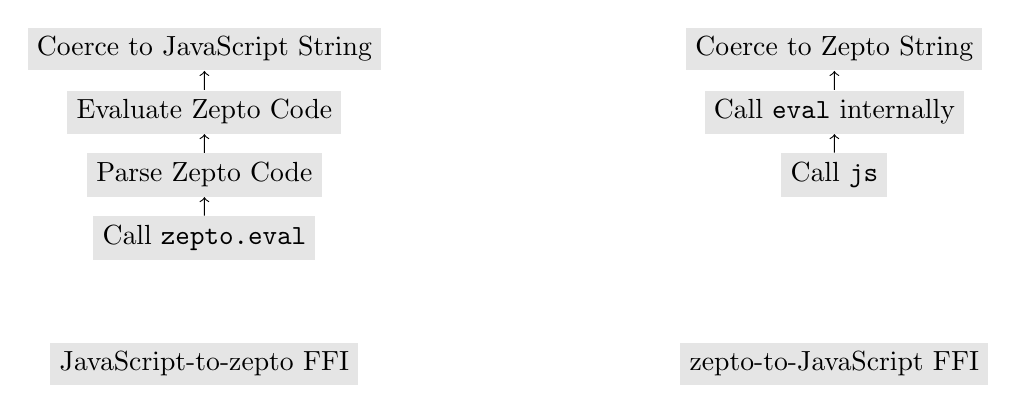
\begin{tikzpicture}
[->,scale=.8,auto=left,every node/.style={rectangle,fill=gray!20}]
  \node (n3) at (5,5)   {Coerce to JavaScript String};
  \node (n2) at (5,4)   {Evaluate Zepto Code};
  \node (n1) at (5,3)   {Parse Zepto Code};
  \node (n0) at (5,2)   {Call \texttt{zepto.eval}};
  \node (descrip0) at (5,0)   {JavaScript-to-zepto FFI};

  \foreach \from/\to in {n0/n1,n1/n2,n2/n3}
    \draw (\from) -> (\to);

  \node (n6) at (15,5)   {Coerce to Zepto String};
  \node (n5) at (15,4)   {Call \texttt{eval} internally};
  \node (n4) at (15,3)   {Call \texttt{js}};
  \node (descrip1) at (15,0)   {zepto-to-JavaScript FFI};

  \foreach \from/\to in {n4/n5,n5/n6}
    \draw (\from) -> (\to);
\end{tikzpicture}
\label{fig:graph}
\end{figure}

\subsection{The \gls{dom}}
\label{sec:DOM}

After building the \gls{ffi}, it was possible to implement the entire
communication with the \gls{dom} in terms of calls to foreign functions
and the parsing of their return values. This allows for a stable library,
because it is unintrusive and does not interfere with existing JavaScript
constructs.

While wrapping the entire \gls{dom} \gls{api} would be a big task, making
the most integral features of the \gls{w3c}'s specifications work turned
out to be rather simple. A minimalistic example of a zepto module
that implements the creation, insertion, and retrieval of elements into
and from the \gls{dom} is presented in Listing \ref{fig:dom}. A production-ready
module would require a host of other features, some of which are already
implemented in a library geared toward zepto-js.

\begin{listing}[H]
\caption{A minimal DOM module.}
\begin{minted}[linenos]{racket}
(module "dom"
  (export
    `("create" ,create)
    `("insert" ,insert)
    `("get" ,get))

  (loads "html")

  (update-dom! (lambda (node contents)
    (js (++ "document.getElementById('" node "').innerHTML = '"
            (create contents)
            "';"))))

  (create (lambda (tree)
    ((import "html:build") tree)))

  (insert (lambda (context tree)
      (update-dom! context tree)))

  (get (lambda (node)
    ((import "html:parse")
       (js (++ "document.getElementById('" node "');"))))))
\end{minted}
\label{fig:dom}
\end{listing}

The \gls{dom} module is not included in the standard library of zepto-js,
as it was too prototypical to be included in a base set of stable
functions. It is, however, available as a third-party \gls{zeps} package
simply called \textit{dom}.\footnote{Should \gls{zeps} be installed on
the target system, it can be installed by issuing \textit{zeps install
hellerve/dom}.} Due to its alpha status it had not yet been registered
to the \gls{zpr} at the time of writing.

\subsection{Language definitions}
\label{sec:LangDef}

One of zepto's most advanced features is language definitions, inspired by
the parser macro system in Racket \parencite{RPM}. Language definitions allow
for a custom parser to be injected into the loading of source files that replaces
zepto's standard parser. These parsers are regular functions that take a string
representing the program as input and emit regular S-Expressions that can be evaluated
as output.\footnote{An example language implementing JSON is presented in Listing \ref{fig:json}.}
This allows for the creation of \glspl{dsl} and other abstractions.
While this is handled fairly differently in zepto than in Racket, the syntax of the
resulting language is compatible. zepto handles the custom parser step with a dispatch
at the time of file loading, which enabled the system to be implemented without
changes to the core language, completely in zepto itself. While this was
designed with portability in mind and thought to ease the transition to
different backends, it actually proved to complicate matters in the case
of the JavaScript port. Here, the module loading system is not present due
to the absence of files in the traditional sense, which made determining where to
plug in the parser dispatcher a problem.

\begin{listing}[H]
\caption{An example language definition that allows for inlining of JSON code.}
\begin{minted}[linenos]{racket}
; json-lang.zp
(load "json/json")

(zepto:implements-lang json:parse "json")

; an example for a file that can now be loaded normally
; it will return a hashmap type
#lang json
{
  "hello": "json"
}
\end{minted}
\label{fig:json}
\end{listing}

As the detection of what to parse is handled from within JavaScript --- by the
MutationObserver mentioned in Section \ref{sec:MutObs} --- the first implementation
of the dispatch mechanism was written entirely in JavaScript. This rendered
the dispatch mechanism relatively clumsy, because registering
additional languages had to be done in JavaScript, making this feature
a JavaScript rather than a zepto feature. While building a parser dispatch
mechanism for JavaScript would certainly also make for an interesting experiment,
it is outside  of the scope of this thesis and would not be a unique feature
to zepto.\footnote{The code for the JavaScript version was salvaged for posteriority
and can be found on \href{https://github.com/hellerve/js-parse-dispatch}{Github under
the name of \texttt{js-parse-dispatch}}.}

This feature was finally dropped altogether from the initial prototype,
as it would either require the impure solution described above or extensive rewrites
of the zepto system --- at least the \texttt{load} statement would require hijacking.
Both of these options incurred too high a maintenance cost for a feature that is
mostly of importance in the context of file-based systems. At the time of writing it
was determined that the implementation of this feature should be deferred to the point
at which the need for other languages or \glspl{dsl} within zepto-js arises.

\setchapterpreamble[u]{%
  \dictum[\emph{R. Buckminster Fuller}]{When I'm working on a problem, I never think about beauty. I think only how to solve the problem. But when I have finished, if the solution is not beautiful, I know it is wrong.}
  \bigskip}
\chapter{Evaluation of the Prototype}
\label{chap:evaluation}

zepto has a small but active user base. Most of these users work with zepto
not in production systems, but as a test environment in which they rapidly
prototype and develop architectures before switching to more mature programming
languages.

This means that developer productivity is more important in the evaluation of
zepto-js than execution speed. Nonetheless, both usability and efficiency
were measured and evaluated. The results are presented in the following.

\section{Usability}

There are many ways to measure usability\footnote{For a comparison of ways
to measure usability of designs, please refer to ``Methods for Measuring
Usability'' \parencite{USBL}.}. All of them come with their own unqiue set
of conveniences and drawbacks. A classical approach from the field of
user-centered software design was chosen for zepto-js --- an alpha test
followed by user feedback.

The changes and their effects on programming in zepto-js were discussed in
a series of rather informal meetings with zepto collaborators, colleagues,
and friends. After a brief introduction, the users were left to their own
devices and their activity was monitored. An overview of their familiarity
with programming for the Web and programming in zepto is given in Figure
\ref{fig:attendees}. For the sake of anonymity their names have been replaced
by numbers. The workshop was conducted on two different days with two different
sets of attendees. On the first day, attendees three, four, and seven were present;
on the second day, attendees one, two, five, and six worked through the material.

While a sample size of seven is clearly suboptimal and not representative
of the diverse background of programmers in general, it provided valuable
insight into how beginners of different knowledge levels approach
programming problems and which parts of zepto-js are cause for confusion.

\begin{figure}
\centering
  \begin{tabu}{| l | l | l | l | l | l | l | l |}
  \hline
  \rowfont{\footnotesize}
  Attendee                        & 1 & 2 & 3 & 4 & 5 & 6 & 7 \\ \hline
  \rowfont{\footnotesize}
  Experience with zepto           & x & x & x & x &   &   &   \\ \hline
  \rowfont{\footnotesize}
  Experience with Web Development &   &   &   & x & x & x &   \\ \hline
  \end{tabu}
  \caption{An overview of the workshop attendees and their experience with zepto and Web Development}
\label{fig:attendees}
\end{figure}

The goal of the workshop was to program an interactive website that would
render personal information in the browser and provide the user with the means
to edit them. This required form handling, validation, and, optionally, the
use of \gls{ajax} technology\footnote{\gls{ajax} is a technique for asynchronous
web applications. It leverages small, data-driven requests instead of the reload
of an entire web page.}. The attendees were provided with a minimal development
template and instructions on how to work with the \gls{ffi} and \gls{dom} in zepto-js.

During the workshops, most questions asked were about tooling and the \gls{ffi}.
Most questions about tooling were asked by those attendees who did know about
web programming, but not about zepto. A conversation with those two attendees
revealed this might be due to them typically relying on build tools to make
their code production-ready, whereas others did not expect that to be included.
Notable here was that attendee four, who had experience with both zepto and Web
Development, did not ask many of these questions, due to the attendee's familiarity
with \gls{zeps} and the zepto ecosystem.

The \gls{ffi} proved to be a recurring source of problems, especially for the
people who did know about zepto, but not about Web Development, as they did not
find proper ways to encode and decode values from and to JavaScript. One of the
goals of further development on zepto-js is thus the inclusion of a library that
simplifies this process.

Tthe users' response to the prototype was, in toto, very positive. Some
of the attendees even suggested they might want to work on it, or with it, on
a regular basis. All, however, except for attendee number seven\footnote{Attendee
number seven had no prior programming experience and was thus very hesitant to
provide comprehensive feedback.}, indicated that it is very obviously a prototypal
system.

Due to time constraints it was not possible to incorporate all of the feedback into
the version of zepto-js described in this thesis. One of the goals moving forward, though,
is to resolve the issues that were present during the workshops. A comprehensive
and intuitive set of documentation, which is currently undergoing finalization, should
also aid in the process of getting started and productive with the language.

\section{Efficiency}

As detailed in Chapter \ref{chap:Implementation}, a lot of adjustments have been made
to make zepto-js as similar to zepto as possible while still providing a sensible \gls{api}
for web development.

Rhe performance of zepto-js against zepto will be measured in the following.
To this end, it  changes will first be summarized and then a few different
benchmarks will be run to determine how the port affects the speed of zepto
code.

\subsection{Additions and Removals}

The \gls{ffi} is a useful addition to bridge the gap between zepto-js and its
environment. It is, however, not present in the reference implementation of zepto.
This is largely due to portability issues with a native foreign function interface;
programs relying on the structure of the underlying execution engine are inherently
unportable unless the architectures of the source and target engine are similar to
each other. The addition of the \gls{ffi} in zepto-js incurs the cost of having to
maintain two very similar but disparate code bases. Without it, the value of a
JavaScript implementation of zepto would not be as apparent.

Features that were removed include the \texttt{load} statement, \gls{repl} functionality,
and language definitions as described in Section \ref{sec:LangDef}. These features
are all interrelated and were dropped because zepto-js does not work on a file-based
system\footnote{This matter was discussed in the Section \ref{sec:LangDef}.}. Zepto-js
uses the tag-based approach presented in Section \ref{sec:MutObs} to fit into the web
ecosystem.

These changes should not affect the performance of zepto-js. The internals of the
interpreters have largely remained the same.

\subsection{Performance measurements}

The largest deciding factor over the performance was expected to be the difference
between a statically compiled binary and a \gls{jit}-compiled or interpreted
JavaScript system. As GHCJS is merely a backend to the \gls{ghc} compiler, the
same optimizations are in place for both.\footnote{Optimizations in \gls{ghc} happen
before the final code generation step. \gls{ghc} utilizes a custom \gls{ir} called
CoreSyn --- described in \cite{CORE} --- on which it performs a lot of optimizations,
for instance inlining as described in \cite{SECR}. There is one caveat, however, which
is also mentioned in \cite{CORE} and that is the compilation to \gls{llvm}, which will
then perform optimizations of its own on the compilate.} Thus, any noticable speed difference
should not be due to zepto.

A small testbench of test programs was written, testing operations on
different data types and of different complexity, from integer addition and
the generation of lists to the calculation of Fibonacci numbers\footnote{Of interest
might be that not the usual tree-recursive algorithm was used but rather the
algorithm that uses the formula \(f(n) = \lfloor{((1 + \sqrt{5}) / 2)^n / \sqrt{5} + 1/2)}\rfloor\),
as found in zepto's standard library. It is of logarithmic time complexity.}.
The example programs are listed in Appendix \ref{app:testbench}, a graphical
representation of the results is provided in Figure \ref{fig:benchres}. The
benchmarking library used is \texttt{bench} from zepto's standard library,
a simplistic benchmarking library for small code snippets. The time it takes to
create the fixture data in the tests was not excluded from the benchmark, as
\texttt{bench} does not include any facility to do so. Even so, the results look
fairly conclusive and were thus deemed appropriate for an analysis of the
prototype.

The benchmarks hint at a small difference in speed, where the reference
in zepto usually takes the lead. An investigation of the counterexample of
hashmap access revealed that the higher performance is due to the JavaScript
engine of the test system --- the most recent version of the Firefox Web browser
that was available at the time of writing --- optimizing for property access, as
this is one of the more common operations in the JavaScript setting \parencite{JSPA}.
As hashmaps compile into a safer version of a data-only JavaScript object, this
optimization takes full effect. Even so, the difference is never bigger than 18\%,
more often than not even under 10\%, making it not significant enough
for exhaustive inspection.

These initial tests seemed to hint at a confirmation of the hypothesis: code executed
in zepto and zepto-js does not vary greatly in performance. These findings notwithstanding,
the final confirmation of that assumption was not possible using exclusively small and
relatively trivial code samples.

It was thus decidded to tackle a more computation-intensive problem:
encoding four Megabytes of random data in Base64\footnote{Base64 is a scheme
for encoding binary as text. It restricts the set of output characters to
sixty-four characters that are both human-readable and URL-safe.}. This
process requires a lot of bitwise operations and string concatentations,
providing a good complement to the benchmarks presented in Figure
\ref{fig:benchres} above.

\begin{figure}[H]
  \begin{subfigure}{.5\textwidth}
  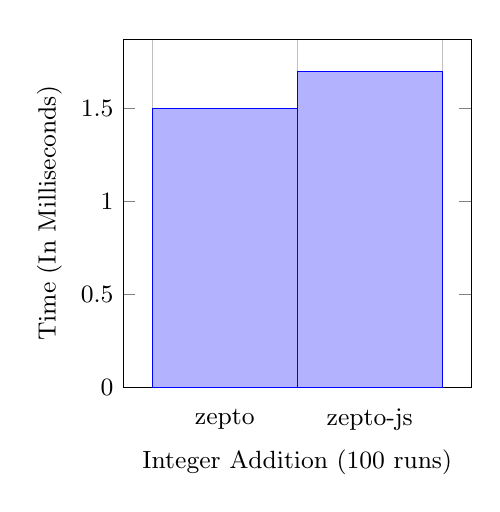
\begin{tikzpicture}[font=\small]
    \begin{axis}[ybar interval,
                 ymin=0,
                 xtick style={draw=none},
                 height=6cm,
                 width=6cm,
                 ylabel=Time (In Milliseconds),
                 xlabel=Integer Addition (100 runs),
                 symbolic x coords={zepto,zepto-js,1}]
      \addplot coordinates {
        (zepto,1.5)
        (zepto-js,1.7)
        (1,0)
      };
    \end{axis}
  \end{tikzpicture}
  \end{subfigure}
  \begin{subfigure}{.5\textwidth}
  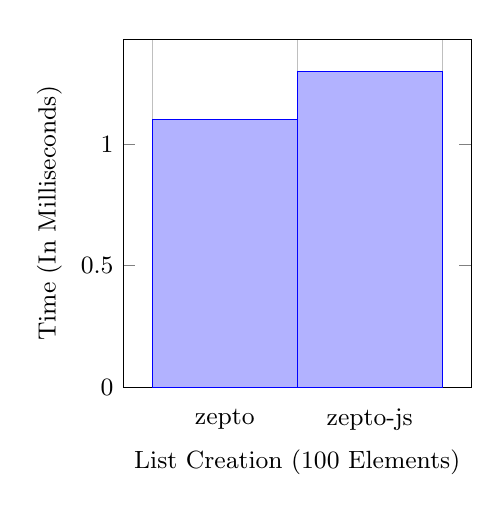
\begin{tikzpicture}[font=\small]
    \begin{axis}[ybar interval,
                 ymin=0,
                 xtick style={draw=none},
                 height=6cm,
                 width=6cm,
                 ylabel=Time (In Milliseconds),
                 xlabel=List Creation (100 Elements),
                 symbolic x coords={zepto,zepto-js,1}]
      \addplot coordinates {
        (zepto,1.1)
        (zepto-js,1.3)
        (1,0)
      };
    \end{axis}
  \end{tikzpicture}
  \end{subfigure}
  \begin{subfigure}{.5\textwidth}
  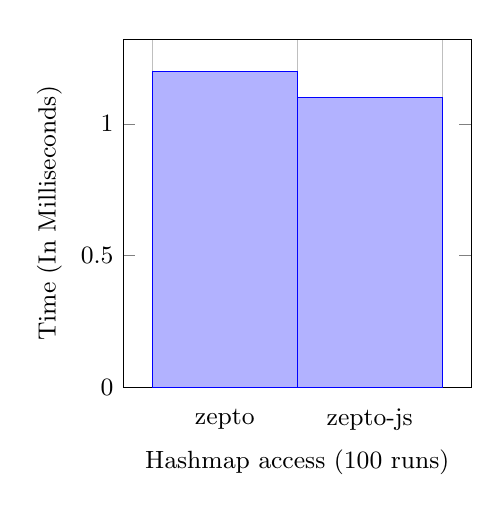
\begin{tikzpicture}[font=\small]
    \begin{axis}[ybar interval,
                 ymin=0,
                 xtick style={draw=none},
                 height=6cm,
                 width=6cm,
                 ylabel=Time (In Milliseconds),
                 xlabel=Hashmap access (100 runs),
                 symbolic x coords={zepto,zepto-js,1}]
      \addplot coordinates {
        (zepto,1.2)
        (zepto-js,1.1)
        (1,0)
      };
    \end{axis}
  \end{tikzpicture}
  \end{subfigure}
  \begin{subfigure}{.5\textwidth}
  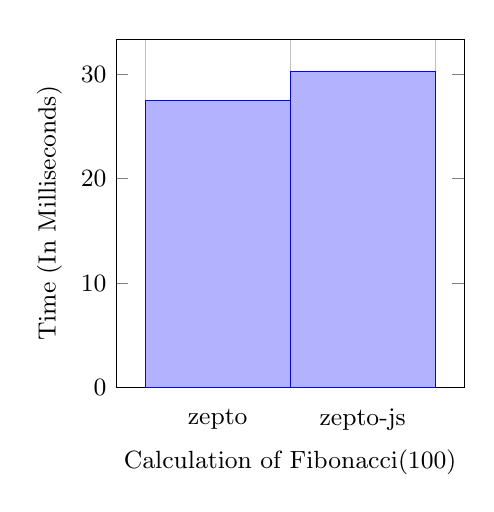
\begin{tikzpicture}[font=\small]
    \begin{axis}[ybar interval,
                 ymin=0,
                 xtick style={draw=none},
                 height=6cm,
                 width=6cm,
                 ylabel=Time (In Milliseconds),
                 xlabel=Calculation of Fibonacci(100),
                 symbolic x coords={zepto,zepto-js,1}]
      \addplot coordinates {
        (zepto,27.5)
        (zepto-js,30.3)
        (1,0)
      };
    \end{axis}
  \end{tikzpicture}
  \end{subfigure}
  \caption{Benchmark comparisons of zepto and zepto-js}
  \label{fig:benchres}
\end{figure}

The tests use zepto's \texttt{base64} library, which is not part of the
standard distribution, but can be installed using \gls{zeps}. This library
is written purely in unoptimized zepto and thus relatively slow. Encoding four
megabytes of binary data takes around one minute in both zepto implementations.
Using the \gls{dom} function \texttt{window.btoa}, however, a standardized function
to encode data in Base64, the execution time  can be dramatically reduced, as shown
in Figure \ref{fig:base64}\footnote{It is denoted as ``zepto-js \gls{ffi}''.}. This
is partly due to the JavaScript function being a natively implemented function rather
than part of a JavaScript library. It should be noted, however, that native JavaScript
code is more often than not faster than its zepto-js equivalent.

\begin{figure}
\centering
  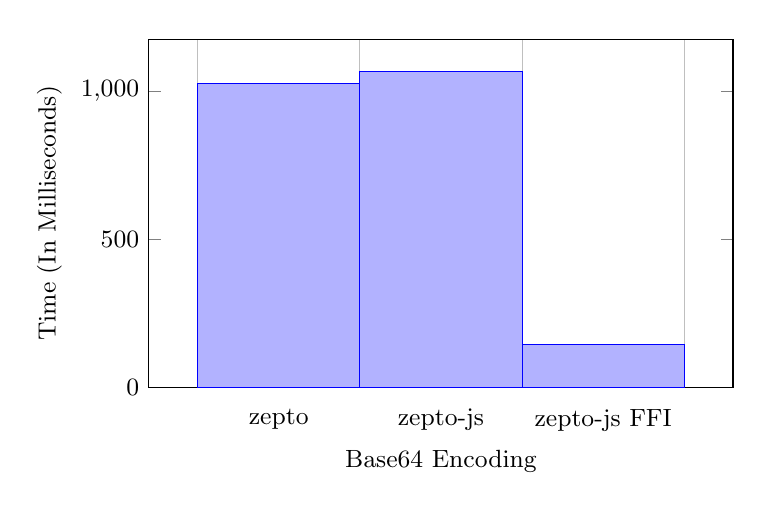
\begin{tikzpicture}[font=\small]
    \begin{axis}[ybar interval,
                 ymin=0,
                 xtick style={draw=none},
                 height=6cm,
                 width=9cm,
                 ylabel=Time (In Milliseconds),
                 xlabel=Base64 Encoding,
                 symbolic x coords={zepto,zepto-js,zepto-js FFI,1}]
      \addplot coordinates {
        (zepto,1023.4)
        (zepto-js,1066.3)
        (zepto-js FFI, 144.1)
        (1,0)
      };
    \end{axis}
  \end{tikzpicture}
  \caption{Measured time when Base64-encoding four Megabytes of data.}
  \label{fig:base64}
\end{figure}

This serves as a good example of how the zepto-js \gls{ffi} can be useful while
also showing that there is room for improvement in the performance of zepto as
a language.

\subsection{Conclusion}

zepto-js is not a language built for speed. This is rather obvious when looking
at the benchmarks provided above. However, by deferring performance-critical code
to the \gls{ffi} and handling tasks that are more easily expressed in zepto ---
big number arithmetic\footnote{For an explanation of zepto's concept of big number
artihmetic, please refer to Section \ref{numbers}.} and metaprogramming come to
mind, among others ---, clean, concise, and fast programs can be generated.

\setchapterpreamble[u]{%
  \dictum[\emph{Isaac Asimov}]{Part of the inhumanity of the computer is that, once it is competently programmed and working smoothly, it is completely honest.}
  \bigskip}
\chapter{Summary and Outlook}
\label{chap:outlook}

The prototype presented in this thesis was never expected to be a replacement
for technologies that are currently making the web what it is. It is a simple
experiment that happens to work well enough to power fewer than a handful of
actual production systems, a blessing for the development of zepto. The
use cases provided real insight into the discrepancy of how the program
works and how it should work. It is also a liability going forward, as users
do not generally appreciate breaking changes.

The software system certainly proved that it is possible to make other
languages work on the web, an idea that is nascent but, by the hopes of
those involved in the production of zepto-js, one that might become a trend
going forward.

Other developments in the zepto ecosystem are just as exciting. There have
been efforts to port zepto to a few different platforms, all of which are
far from finished. Nonetheless, it has been interesting to follow their development.
The compiler and parser have both gained language implementations, some of
them usable --- the aforementioned compiler backends for LLVM and Erlang come to
mind, as well as a web server framework that uses a \gls{dsl} to simplify writing
request handlers ---, some of them borne purely out of the desire to toy around
with the language; parsers and cross-compilers have been written for a handful of
esoteric programming languages, including Brainfuck\footnote{Brainfuck is a language
that aims to reduce programming to its most minimal form and tries to emulate a Turing
machine \parencite{BFK}.}, Io, and Iota\footnote{Io and Iota are conceptually similar
to Brainfuck, although they try to reduce programming to the lambda calculus described
by Alonzo Church \parencite{IOT}.}.

The development of \gls{zeps} has surely contributed to the growth of zepto and
fueled the development of zepto-js. It is tested on real systems and has
withstood the scrutiny of colleagues and contributors. By the definition of the
development team, however, it is not yet ready for a big public release, hence
the timid version number of 0.0.7. A stable version might not be as far in the
distance as this number suggests, but it certainly is far enough away to merit
a healthy dose of defensiveness.

Another big development in the zepto community has certainly been a series of
classes and workshops. They too helped route the development of zepto down
a path of usability, self-awareness, and constant reevaluation. Targeted at an
audience of diverse people with mostly little to no experience with functional
programming or Lisp, the workshops have shown to not only awaken an interest in those
concepts. They also led to the development of a few projects for zepto and its
JavaScript-backed counterpart that now have become part of the standard toolset,
such as the plugins for the Atom\footnote{Atom is an editor that was developed by
the Github team as a lightweight, powerful, and pluggable development environment
\parencite{ATOM}.} and Vim\footnote{Vim is the standard editor for the command line
of most Linux distributions \parencite{VIM}.} editors.

In regard to tooling for zepto-js, a newly formed development team, comprised of
people experienced in web development, is building plugins for zepto-js to integrate
with Gulp\footnote{One of the tools mentioned in Section \ref{sec:IntegrationTooling}.} for
tasks like minification and dependency resolution. Integration of \gls{zeps} with
Gulp is a subject for the near future too.

All of these developments start to hint at a community in its nascence. It might
be too soon to judge whether or not this is true, but it would certainly be a welcome
development for zepto and its maintainers.

\chapter{Conclusion}
\label{chap:conclusion}

There have been voices that have insisted that the web need be fixed
since its inception. Most disagreements over its inner workings
have been philosophical and are a matter of ongoing dispute.
While the web certainly can be improved --- like any system,
at any time --- I do not believe it is fundamentally flawed. The
technologies that power the current World Wide Web, from switches
and cable technologies to protocols and development frameworks,
have shown to be robust enough for a large part of the world
to interconnect. We steadily adapt the way we work with it
as trends and paradigms emerge and evolve.

One of the major redeeming qualities of the fundamental
philosophies of the World Wide Web has certainly been
its ability to adapt to changes. Standardization of web
technologies has a reputation for being slow, but in terms
of design processes on a global scale, it is actually reasonably
fast.

zepto is a young language that has adopted this mindset ---
it changes rapidly and a stable release has yet to be announced.
With this thesis, an important step towards reaching a fulfillment
of its design goals has been taken.

Many questions addressed by this thesis remain unanswered.
Even with that in mind, I hope that my work has asked
questions that are worth being asked and that the technologies
presented in this thesis will allow for more technologies to
come to the web, so that an even more heterogeneous,
expressive, and inclusive system can emerge, one that
caters to different aesthetics, philosophies, and mindsets.

I would happily welcome any contributions towards that
end, both related and unrelated to the technology
that is zepto.


%============================================
%============================================
% end matter

\appendix

\chapter{List of Modules in the zepto Standard Library}
\label{app:stdlib}

Libraries that are loaded by default are denoted by \textit{(dflt.)}.

\begin{description}
\item [argparse] A command line argument parser
\item [ascii] An ASCII art modul
\item [bench] A simple benchmarking and timing library
\item [calculus] A library that implements combinators of the lambda calculus
\item [char\textit{(dflt.)}] A library of functions for working with characters
\item [cl] A library that exports standard Common Lisp functions
\item [data] A library that exports lazy data types, such as queues, deques and streams
\item [datetime] A library for working with and formatting dates and times
\item [delay\textit{(dflt.)}] A utility library for delaying computations
\item [infix] A library that translates infix mathematical expressions to the appropriate
prefix form
\item [io\textit{(dflt.)}] A library of functions for Input and Output
\item [json] A JSON parser and renderer
\item [keywords\textit{(dflt.)}] A library that allows for keyword arguments as found in Python
\item [marsaglia] A library of functions for cryptographically strong Pseudo-Random Number Generators
\item [math\textit{(dflt.)}] A library of functions for mathematical purposes
\item [minitest] A testing library
\item [module\textit{(dflt.)}] zepto's module system
\item [monads] A library of monads and monadic computations
\item [parsecomb] A parser combinator library
\item [pointfree] A library for defining functions in point-free style
\item [querystring] A querystring parser and renderer
\item [random\textit{(dflt.)}] A library of functions for cryptographically insecure random number
and data generation
\item [rsa] A RSA library
\item [slugify] A library for generations slugs
\item [sort\textit{(dflt.)}] A sorting library
\item [srfi\textit{(dflt.)}] A library of SRFIs
\item [statistics] A statistics library
\item [struct\textit{(dflt.)}] A library for generating structs with the appropriate functions
declaratively
\item [zpbash] A BASH library
\item [zpcllections\textit{(dflt.)}] A library of functions for defining and working with collections
\item [zpcont\textit{(dflt.)}] A library of functions for working with continuations
\item [zpconversion\textit{(dflt.)}] A library of functions for converting between datatypes
\item [zperror\textit{(dflt.)}] A library of functions for working with errors
\item [zpfile\textit{(dflt.)}] A library of functions for working with files
\item [zpgenerics\textit{(dflt.)}] A library of functions for defining and working with
generic functions
\item [zphash\textit{(dflt.)}] A library of functions for working with hash maps
\item [zplist\textit{(dflt.)}] A library of functions for working with lists
\item [zpnumbers\textit{(dflt.)}] A library of functions for working with numerical values
\item [zpstring\textit{(dflt.)}] A library of functions for working with strings
\item [zpvector\textit{(dflt.)}] A library of functions for working with vector
\item [zpversion\textit{(dflt.)}] A library of functions for working with the current zepto version
\end{description}

\chapter{List of \gls{zeps} commands}
\label{app:zepscmds}

This list can also be found in the README of zeps under
\texttt{https://github.com/zeps-system/zeps}.

\begin{description}
\item [test] Runs the module tests.
\item [t] shortcut for test.
\item [search] Search for packages matching a search term (on the ZPR).
\item [sandbox] Create/destroy a sandboxed zeps environment
\item [run] Run the module entry-point, without installing it
\item [repl] Launches an interactive shell with a certain module preloaded.
\item [remove] Removes a package.
\item [rm] shortcut for remove.
\item [register] Registers a package.
\item [r] shortcut for register.
\item [new] Bootstraps a new package.
\item [n] Shortcut for new.
\item [keygen] Generates a new RSA key for zeps.
\item [install] Installs a package.
\item [i] Shortcut for install.
\item [help] Interactive help on getting started
\item [readme] Prints zeps' README
\end{description}

\chapter{The programs used in zepto-js' benchmarks}
\label{app:testbench}

The programs presented here aim to be fairly simple and
self-contained.

\begin{listing}[H]
\caption{Integer Addition}
\begin{minted}[linenos]{racket}
  (load "bench/bench")
  (import-all "bench")

  (bench:bench [+ 100 1] 100)
\end{minted}
\end{listing}

\begin{listing}[H]
\caption{List Creation}
\begin{minted}[linenos]{racket}
  (load "bench/bench")
  (import-all "bench")

  (bench:bench [range 100] 1)
\end{minted}
\end{listing}

\begin{listing}[H]
\caption{Hashmap Access}
\begin{minted}[linenos]{racket}
  (load "bench/bench")
  (import-all "bench")

  (bench:bench [#{:x 10 :y 12} :x] 100)
\end{minted}
\end{listing}

\begin{listing}[H]
\caption{Calculation of Fibonacci(100)}
\begin{minted}[linenos]{racket}
  (load "bench/bench")
  (import-all "bench")

  (bench:bench [math:fib 100] 1)
\end{minted}
\end{listing}

The following example represents the Base64-encoding of data.
It assumes that there is a file called ``data.dat'' that holds
the data to be encoded. It will only work in the reference
implementation of zepto.

\begin{listing}[H]
\caption{Base64 for zepto}
\begin{minted}[linenos]{racket}
  (load "bench/bench")
  (load "base64/base64")

  (import-all "bench")
  (import-all "base64")

  (bench:bench `(base64:encode ,(read-contents-binary "data.dat")) 1)
\end{minted}
\end{listing}

The zepto-js version is included below. It assumes the data
is contained in a HTML tag with the ID ``data''.

\begin{listing}[H]
\caption{Base64 for zepto-js}
\begin{minted}[linenos]{racket}
  (load "bench/bench")
  (load "base64/base64")

  (import-all "bench")
  (import-all "base64")

  (define fixture (js "document.getElementById('#data').innerHTML"))

  (bench:bench `(base64:encode ,fixture) 1)
\end{minted}
\end{listing}

The version that leverages the \gls{ffi} is presented below.

\begin{listing}[H]
\caption{Base64 for zepto-js, using the \gls{ffi}}
\begin{minted}[linenos]{racket}
  (load "bench/bench")
  (import-all "bench")

  (define fixture (js "document.getElementById('#data').innerHTML"))

  (bench:bench `(js (++ "window.btoa('" ,fixture "')")) 1)
\end{minted}
\end{listing}


\backmatter

\bookmarksetup{startatroot}

\printbibliography[title=References,heading=bibintoc]

\clearpage

\begin{minipage}{1.0\textwidth}
  \begin{center}
    \vspace{5cm}
    \LARGE \textbf{Eigenständigkeitserklärung}
  \end{center}

  \vspace{2cm}
  \normalsize
Hiermit versichere ich, dass ich die vorliegende Bachelorarbeit selbstständig
und nur unter Verwendung der angegebenen Quellen und Hilfsmittel verfasst habe.
Die Arbeit wurde bisher in gleicher oder ähnlicher Form keiner anderen Prüfungsbehörde
vorgelegt.
  \vspace{1cm}
  \par\noindent\makebox[2.5in]{\hrulefill}     \hfill\makebox[2.0in]{\hrulefill}%
  \par\noindent\makebox[2.5in][l]{Veit Heller} \hfill\makebox[2.0in][l]{Ort, Datum}%

\end{minipage}

\end{document}
